%%%%%%%%%%%%%%%%%%%%%%%%%%%%%%%%%%%%%%%%%
% Short Sectioned Assignment
% LaTeX Template
% Version 1.0 (5/5/12)
%
% This template has been downloaded from:
% http://www.LaTeXTemplates.com
%
% Original author:
% Frits Wenneker (http://www.howtotex.com)
%
% License:
% CC BY-NC-SA 3.0 (http://creativecommons.org/licenses/by-nc-sa/3.0/)
%
%%%%%%%%%%%%%%%%%%%%%%%%%%%%%%%%%%%%%%%%%

%----------------------------------------------------------------------------------------
%	PACKAGES AND OTHER DOCUMENT CONFIGURATIONS
%----------------------------------------------------------------------------------------

\documentclass[paper=a4, fontsize=11pt]{scrartcl} % A4 paper and 11pt font size

\usepackage[T1]{fontenc} % Use 8-bit encoding that has 256 glyphs
%\usepackage{fourier} % Use the Adobe Utopia font for the document - comment this line to return to the LaTeX default
\usepackage[english]{babel} % English language/hyphenation
\usepackage{amsmath,amsfonts,amsthm} % Math packages
\usepackage{mathtools} %More math! (For dscases)
\usepackage{hyperref} %HTML package
\usepackage{pgfplots} %Makes plots in LaTeX
\usepackage{tikz} %Also tikz?
\usepackage{bm} %makes vectors bold
\usepackage{bbm} %Blackboard bold 1
\usepgfplotslibrary{fillbetween}%Let's me fill between named plots
\usepackage{graphicx} %import pics

\usepackage[noend]{algpseudocode} %Algorithms
\usepackage{algorithm}

\graphicspath{ {Python\_figs/} }
\DeclareGraphicsExtensions{.pdf,.png,.jpg}
\usepackage{sectsty} % Allows customizing section commands
\allsectionsfont{ \normalfont\scshape} % Make all sections the default font and small caps


\renewcommand{\thesubsection}{\alph{subsection}} %Make subsections start with letters

\usepackage{fancyhdr} % Custom headers and footers
\pagestyle{fancyplain} % Makes all pages in the document conform to the custom headers and footers
\fancyhead{} % No page header - if you want one, create it in the same way as the footers below
\fancyfoot[L]{} % Empty left footer
\fancyfoot[C]{} % Empty center footer
\fancyfoot[R]{\thepage} % Page numbering for right footer
\renewcommand{\headrulewidth}{0pt} % Remove header underlines
\renewcommand{\footrulewidth}{0pt} % Remove footer underlines
\setlength{\headheight}{13.6pt} % Customize the height of the header

\numberwithin{equation}{section} % Number equations within sections (i.e. 1.1, 1.2, 2.1, 2.2 instead of 1, 2, 3, 4)
\numberwithin{figure}{section} % Number figures within sections (i.e. 1.1, 1.2, 2.1, 2.2 instead of 1, 2, 3, 4)
\numberwithin{table}{section} % Number tables within sections (i.e. 1.1, 1.2, 2.1, 2.2 instead of 1, 2, 3, 4)

\setlength\parindent{0pt} % Removes all indentation from paragraphs - comment this line for an assignment with lots of text

\usepackage{tikz}
\usetikzlibrary{positioning}
\usepackage{placeins}

\usepackage{listings}
\lstset{language=Python}

\usetikzlibrary{arrows,automata}
\usetikzlibrary{positioning}

\tikzstyle{arn_n} = [circle, white, font=\bfseries, draw=black, fill=black, align=center, inner sep=0pt,text width=1.5em, text centered]% black node
\tikzstyle{arn_r} = [circle, red, draw=red, align=center, inner sep=0pt,text width=1.5em, text centered, very thick]% red node
\tikzstyle{arn_x} = [rectangle, draw=black, align=center, inner sep=0pt,minimum width=0.5em, minimum height=0.5em]% NIL 'node'


%----------------------------------------------------------------------------------------
%	TITLE SECTION
%----------------------------------------------------------------------------------------

\newcommand{\horrule}[1]{\rule{\linewidth}{#1}} % Create horizontal rule command with 1 argument of height

\title{	Assignment 6}

\author{Benjamin Jakubowski} % Your name

\date{\normalsize\today} % Today's date or a custom date

\begin{document}

\maketitle % Print the title

%----------------------------------------------------------------------------------------
%	PROBLEM 1
%----------------------------------------------------------------------------------------
\section{Non-recursive algorithms for inorder BST traversal}

\subsection{Solution using a stack}

The idea for the in-order BST traversal algorithm using a stack can be summarized simply:
\begin{itemize}
\item Go as far left as you can
\item Once you've gone as far left as you can, you've found the (next) smallest element. Visit (print) it, then move right
\end{itemize}

The algorithm is presented in full below:

\begin{algorithmic}
\Function{inorder\_traversal\_with\_stack}{T}
	\State x = T.root
	\State nodes\_seen = new Stack()
	\While{(len(nodes\_seen) > 0) or (x is not Null)}
		\If{(x is not Null)}
			\State nodes\_seen.push(x)
			\State x = x.left
		\Else
			\State x = nodes.seen.pop()
			\State print x
			\State x = x.right
		\EndIf
	\EndWhile
\EndFunction
\end{algorithmic}

\subsection{Solution without stack, using threading}

Note this algorithm assumes that threads are not already present in the tree (i.e. the threads from leaves to successors are constructed and removed in the course of the algorithm). The algorithm is explained via comments.\\

\begin{algorithmic}
\Function{inorder\_traversal\_without\_stack}{T}
	\State x = T.root
	\While{(x is not Null)}
		\If{(x.left is Null)} \Comment{Then x's successor is its right child}
			\State print x
			\State x = x.right
		\Else \Comment{Check if x's predecessor is already threaded to x}
			\State tmp = x.left \Comment{x's predecessor is right-most leaf of left subtree}
			\While{(tmp.right is not Null) and (tmp.right is not x)}:
				\State tmp=tmp.right 
			\EndWhile
			\If {tmp.right is Null} \Comment{Then no thread from predecessor to x}
				\State tmp.right = x \Comment{Add thread}
				\State x = x.left \Comment{Move from x into its left subtree}
			\Else \Comment{Broke out of while loop with tmp.right == x}
				\State tmp.right = Null \Comment{Thus we've visited x's entire left subtree.}
				\State print x \Comment{Visit (print) x after nulling thread.}
				\State x = x.right \Comment{Move into x's right subtree}
			\EndIf
		\EndIf
	\EndWhile
\EndFunction
\end{algorithmic}

%----------------------------------------------------------------------------------------
%	PROBLEM 2
%----------------------------------------------------------------------------------------
\section{Recursive version of \texttt{Tree-Insert}}

\begin{algorithmic}
\Function{recursive\_insert}{T, z, x = T.root}
	\State \emph{T is tree, z is node to insert, x is starting node for recursive call}
	\State \emph{Note we use default arguments to handle the initial call}
	\If{z is Null}
		\State \Return \Comment{Handles edge case}
	\ElsIf{x is Null} \Comment{Then T.root is Null}
		\State T.root = z
	\ElsIf {z.key < x.key}
		\If {x.left is Null} \Comment{Then insert z as left child of x}
			\State x.left = z
			\State z.parent = x
		\Else \Comment{Then recurse}
			\State recursive\_insert(T, z, x.left)
		\EndIf
	\Else \Comment{Then z.key $\geq$ x.key}
		\If {x.right is Null}\Comment{Then insert z as right child of x}
			\State x.right = z
			\State z.parent = x
		\Else \Comment{Then recurse}
			\State recursive\_insert(T, z, x.right)
		\EndIf
	\EndIf
\EndFunction
\end{algorithmic}

%----------------------------------------------------------------------------------------
%	PROBLEM 3
%----------------------------------------------------------------------------------------
\section{Average depth of node in BST}

Our objective in this problem is to show that the average depth of a node in a randomly built binary search tree with $n$ nodes is $O(\lg n)$.

First, we define the \emph{total path length} $P(T)$ of a binary tree $T$ as the sum, over all nodes $x$ in $T$, of the depth of node $x$, which we denote by $d(x, T)$.

\subsection{Average depth of a node in $T$}

The total path length is
\[P(T) = \sum_{x \in T} d(x, T)\]
Thus, dividing by $\frac{1}{n}$ yields the desired result
\[\frac{1}{n} \sum_{x \in T} d(x, T) = \frac{1}{n} P(T)\]

\subsection{Recursive definition of $P(T)$}

Let $T_L$ and $T_R$ be the left and right subtrees of tree $T$, respectively. We aim to show if $T$ has $n$ nodes, then
\[P(T) = P(T_L) + P(T_R) + n - 1\]

First, note
\[d(x, T_L) = d(x, T) - 1 \qquad{} \textrm{for all } x \in T_L\]
\[d(x, T_R) = d(x, T) - 1 \qquad{} \textrm{for all } x \in T_R\]

Thus,
\begin{align*}
P(T) &= \sum_{x \in T} d(x, T) \\
	&= \sum_{x \in T_L} d(x, T) + \sum_{x \in T_R} d(x, T) + d(x_{root}, T)\\
	&= \sum_{x \in T_L} [d(x, T_L) + 1] + \sum_{x \in T_R} [d(x, T_R) + 1] + 0\\
	&= \sum_{x \in T_L} d(x, T_L) + \sum_{x \in T_R} d(x, T_R) + \underbrace{(n - 1)}_{\textrm{since } n-1 \textrm{ nodes in } T_R + T_L}\\
	&= P(T_L) + P(T_R) + n - 1
\end{align*}

\subsection{Expression for $P(n)$}

Now let $P(n)$ denote the average total path length of a randomly built binary search tree with $n$ nodes. We aim to show that
\[P(n) = \frac{1}{n} \sum_{i = 0}^{n-1} \left(P(i) + P(n - i -1) + n - 1\right)\]

We use induction on $n$ to do so. First, note that $P(0)$ is trivially $0$. Thus, for a base case, we show this expression holds for $P(1)$ (noting in advance a randomly build a tree with $n = 1$ nodes always has a total path length of $0$):
\begin{align*}
P(n = 1) &= \frac{1}{1} \sum_{i = 0}^{1-1} \left(P(i) + P(1 - i -1) + 1 - 1\right) \\
 	&= \left(P(0) + P(1 - 0 -1) + 1 - 1\right) \\
	&= 0
\end{align*}

Next, assume this expression is true for all $k < n$. Now consider a tree with $n$ nodes. Let the $n$ keys in this tree be ordered as
\[k_0, k_1, \cdots, k_{n-1}\]
Then, under the assumption the $n$ keys are inserted into the BST in permuted order, with all permutations equiprobable, the probability the root node (i.e. first key inserted) has key $k_j$ is $\frac{1}{n}$ for all $j \in \{0, 1, \cdots, n-1\}$.

Next, note (given $k_j$  is the root)
\begin{itemize}
\item $T_L$ has $j$ nodes
\item $T_R$ has $n - j - 1$ nodes
\end{itemize}

Thus, (given $k_j$  is the root), by our inductive hypotheses the average total path for this tree is $P(j) + P(n - j -1) + n - 1$.

Finally, to find the average total path length for randomly built $n$ node BST's, we simply take the expectation over $j$, the index of the root key in our ordered set:
\begin{align*}
P(n) &= \sum_{j = 0}^{n-1} P(\textrm{Insert key } k_j \textrm{ first})\left[P(j) + P(n - j -1) + n - 1\right] \\
	&= \sum_{j = 0}^{n-1} \frac{1}{n}\left[P(j) + P(n - j -1) + n - 1\right] \\
	&= \frac{1}{n} \sum_{j = 0}^{n-1} \left[P(j) + P(n - j -1) + n - 1\right]
\end{align*}

\subsection{Rewriting $P(n)$}

We proceed from the expression derived in part (c)

\begin{align*}
P(n) &= \frac{1}{n}\left[\sum_{j = 0}^{n-1} P(j) + \sum_{j = 0}^{n-1} P(n - j -1)\right] + \frac{1}{n}n(n - 1) \\
	&= \frac{1}{n}\left[P(0) + P(1) + \cdots + P(n - 1) + P(n - 1) + P(n - 2) + \cdots + P(0)\right] + \underbrace{(n - 1)}_{\Theta(n)} \\
	&= \frac{2}{n}\underbrace{\sum_{j = 0}^{n-1} P(j)}_{\textrm{Recall } P(0) = 0} + \Theta(n) \\
	&= \frac{2}{n}\sum_{j = 1}^{n-1} P(j) + \Theta(n)
\end{align*}

\subsection{Showing $P(n) = O(n \lg n)$}

First, following CLRS problem 7-3, we show
\[\sum_{k = 1}^{n - 1} k \lg k \leq \frac{1}{2}n^2 \lg n - \frac{1}{8} n^2\]

\begin{align*}
\sum_{k = 1}^{n - 1} k \lg k  &= \sum_{k = 2}^{n - 1} k \lg k \qquad{} \textrm{Since } \lg 1 = 0 \\
	&\leq \sum_{k = 2}^{n} k \lg k \\
	&\leq \int_{k = 2}^{n} k \lg k \textrm{ d}k \qquad{} \textrm{Since } k \lg k > 0 \textrm{ and monotone} \\
	&= \left[\frac{1}{2}k^2 \lg k - \frac{1}{4\ln2}k^2\right]\Bigg|_{k=2}^{k = n}\\
	&\leq \left[\frac{1}{2}k^2 \lg k - \frac{1}{8}k^2\right]\Bigg|_{k=2}^{k = n}\\
	&= \left[\frac{1}{2}n^2 \lg n - \frac{1}{8}n^2\right] - \left[\frac{1}{2}2^2 \lg 2 - \frac{1}{8}2^2\right] \\
	&= \left[\frac{1}{2}n^2 \lg n - \frac{1}{8}n^2\right] - \left[2 - \frac{1}{2}\right] \\
	&\leq \left[\frac{1}{2}n^2 \lg n - \frac{1}{8}n^2\right]
\end{align*}

Next, note for $k = 1, P(k = 1) = 0 \leq 0 = c \cdot 1 \cdot \lg 1$ for any $c > 0$. Now assume for all $k < n$, there exists some $c > 0$ such that
\[P(k) \leq c \cdot k \lg k\]
Then
\begin{align*}
P(n) &= \frac{2}{n}\sum_{j = 1}^{n-1} P(j) + \Theta(n) \\
	&=  \frac{2}{n}\sum_{j = 2}^{n-1} P(j) + \Theta(n) \qquad{} \textrm{Since } P(1) = 0\\
	&\leq \frac{2}{n}\sum_{j = 2}^{n-1} c_j \cdot k \lg k + \Theta(n)
\end{align*}
Now let $c_{\max} = \max\{c_2, \cdots, c_{n -1}\}$. Then
\begin{align*}
P(n) &\leq \frac{2}{n}\sum_{j = 2}^{n-1} c_{\max} \cdot k \lg k + \Theta(n) \\ 
	&\leq \frac{2c_{\max}}{n}\left[\frac{1}{2}n^2 \lg n - \frac{1}{8}n^2\right] + \Theta(n) \\ 
	&= c_{\max} \cdot n \lg n - \frac{c_{\max}}{4} n + \Theta(n)
\end{align*}
Next, let's unpack $\Theta(n)$ (using the implied upper bound $k\cdot n$ for all $n > n_0$).
\begin{align*}
P(n) &\leq c_{\max} \cdot n \lg n - \frac{c_{\max}}{4} n + k \cdot n \qquad{} \forall ~ n > n_0\\
	&= c_{\max} \cdot n \lg n + \left(k - \frac{c_{\max}}{4}\right) n
\end{align*}
Now, note the inequality assumed in the inductive hypothesis

\[P(k) \leq c \cdot k \lg k \leq c_{\max} \cdot k \lg k\]

also holds for any $c' > c_{\max}$. In particular, it holds for $c' \geq \max\{c_{\max}, 4k\}$. But then note

\[\left(k - \frac{c'}{4}\right) n \leq 0\]

This yields the final inequality
\begin{align*}
P(n) 	&= c_{\max} \cdot n \lg n + \left(k - \frac{c_{\max}}{4}\right) n \\
	&\leq c' \cdot n \lg n + \left(k - \frac{c'}{4}\right) n \\
	&\leq c' \cdot n \lg n \qquad{}  \forall ~ n > n_0
\end{align*}

Thus, $P(n) = O(n \lg n)$.

\subsection{An implementation of quicksort with same comparisons as BST}

Consider a random array of $n$ distinct integer elements.
\[A = [a_1, \cdots, a_n]\]
Consider constructing a BST from $A$. Note the root of the tree is the first element inserted in the BST. It is also compared to all other elements in $A$- thus it is the first pivot in our desired quicksort algorithm. 

Similarly, given an internal node $x$
\begin{itemize}
\item $x.left$ is
\begin{itemize}
\item The pivot for the first recursive quicksort call (i.e. the call for all elements in the range \texttt{lo} to \texttt{hi} that are less than $x$).
\item The first element in this range inserted into the BST
\end{itemize}
\item $x.right$ is
\begin{itemize}
\item The pivot for the second recursive quicksort call (i.e. the call for all elements in the range \texttt{lo} to \texttt{hi} that are greater than $x$).
\item The second element in this range inserted into the BST.
\end{itemize}
\end{itemize}

Thus, we can implement quicksort with the same comparisons as BST fairly simply. All we need to do is change how we select the pivot. Recall in vanilla quicksort, the function \texttt{partition(A, lo, hi)} picks \texttt{pivot = A[hi]}. Instead, we pick the element in the range $A[lo, hi]$ inclusive that had the lowest index in the original ordering of  array $A$.

We do so by implementing the following function, which calls a helper function \texttt{original\_index} which gets the original index of \texttt{A[i]}:

\begin{algorithmic}
\Function{put\_pivot\_at\_hi}{A, lo, hi}
	\State original\_index\_of\_pivot = original\_index(A[lo])
	\State current\_index = lo
	\For{i in lo+1, $\cdots$ hi}
		\If{original\_index(A[i]) < original\_index\_of\_pivot}
			\State original\_index\_of\_pivot = original\_index(A[i])
			\State current\_index = i
		\EndIf
	\EndFor
	\State swap(A[i], A[hi])
\EndFunction
\end{algorithmic}

Note this version of the algorithm takes more space, but ensures we make the same comparisons.

%----------------------------------------------------------------------------------------
%	PROBLEM 4
%----------------------------------------------------------------------------------------
\section{Bound on longest simple path in red-black tree}

Let $x$ be a node in a red-black tree. Then, by red-black tree property 5 , the shortest simple path from $x$ to a descendent leaf also has $bh(x)$ black nodes and at least $0$ red nodes. Thus the length of the shortest path is
\[P_{shortest} \geq bh(x)\]

Next consider the longest simple path from $x$ to a descendent leaf. The length of this path is simply the height of $x$, namely $h(x)$. Note the number of black nodes on the path is $bh(x)$. Thus, the number of red nodes on this path is
\[rh(x) = h(x) - bh(x)\]
Now note $rh(x) \leq bh(x)$. This follows by red-black tree property 4 (since every red node in the path is immediately followed by a black node). Thus,
\[h(x) = rh(x) + bh(x) \leq bh(x) + bh(x) = 2 bh(x) \leq 2 P_{shortest}\]

Hence, the length of the longest simple path $h(x)$ is at most twice that of the shortest simple path.

%----------------------------------------------------------------------------------------
%	PROBLEM 5
%----------------------------------------------------------------------------------------
\section{Largest and smallest number of internal nodes}

First, by CLRS page 309, a tree rooted at node $x$ with black-height $bh(x) = k$ has at least $2^k - 1$ internal nodes.

Now for an upper bound on the number of internal nodes. To start, consider a single node tree with key $k_0$.  Note this single node tree has black height 1, and adding two red nodes with keys $k_1$ and $k_2$ such that $k_1 < k_0 < k_2$ does not change the black height. 

\begin{center}
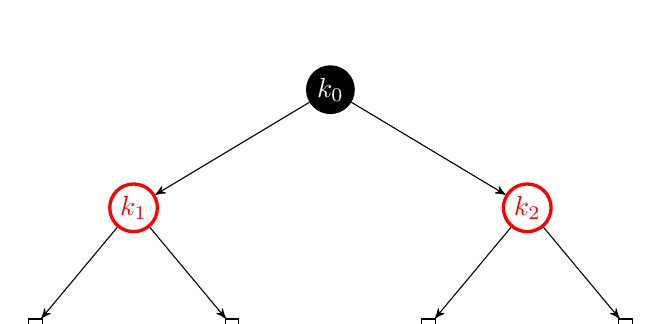
\begin{tikzpicture}[->,>=stealth',level/.style={sibling distance = 5cm/#1, level distance = 1.5cm}] 
\node [arn_n] {$k_0$}
    child{ node [arn_r] {$k_1$}
        child{ node [arn_x] {}}
        child{ node [arn_x] {}}
    }
    child{ node [arn_r] {$k_2$}
        child{ node [arn_x] {}}
        child{ node [arn_x] {}}
    }
; 
\end{tikzpicture}
\end{center}

However, adding any additional nodes increases the black height (since the parents of the $T.nil$ leaf nodes are now all red, so adding additional nodes necessarily requires recoloring and rotating, which increases the black height).

Thus, when the black height is 1, we can have no more than 3 internal nodes. This suggests the bound on $n(T_k)$, the number of internal nodes in a tree $T$ with black-height $k$, of
\[n(T_k) \leq 2^{2k} - 1\]

Now we prove this bound by induction. Assume all trees with black-height $k' < k$ have at most $2^{2k'} - 1$ internal nodes. Now consider a red black tree with black-height k. Note we can construct the tree black-height $k$ with a maximum number of internal nodes such a tree as follows:
\begin{center}
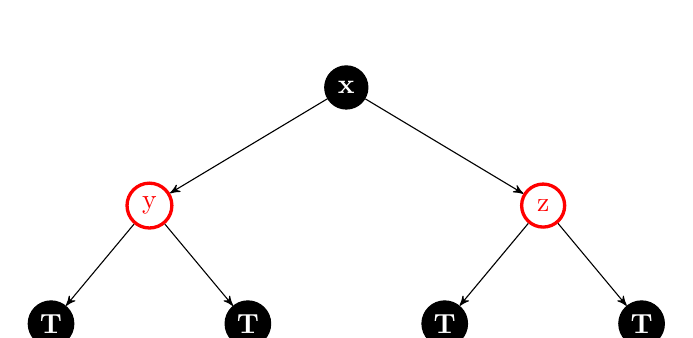
\begin{tikzpicture}[->,>=stealth',level/.style={sibling distance = 5cm/#1, level distance = 1.5cm}] 
\node [arn_n] {x}
    child{ node [arn_r] {y}
        child{ node [arn_n] {T}}
        child{ node [arn_n] {T}}
    }
    child{ node [arn_r] {z}
        child{ node [arn_n] {T}}
        child{ node [arn_n] {T}}
    }
; 
\end{tikzpicture}
\end{center}
where $T$ are subtrees with black-height $k - 1$ and at most $2^{2(k-1)} - 1$ internal nodes.

Then the number of internal nodes in this tree is
\begin{align*}
n(T_k) &\leq 4\cdot (2^{2(k-1)} - 1) + 3 \\
	&\leq 2^2\cdot 2^{2k - 2} - 4 + 3 \\
	&\leq \cdot 2^{2k - 2 + 2} - 1 \\
	&\leq \cdot 2^{2k} - 1
\end{align*}
Thus $n(T_k) \leq 2^{2k} - 1$.

%----------------------------------------------------------------------------------------
%	PROBLEM 6
%----------------------------------------------------------------------------------------
\section{Largest and smallest possible ratio of red to black internal nodes}

Per the hint, we chose to pick a convenient n. Specifically, let's take some $n$ such that
\[n = \sum_{i=0}^k 2^i = 2^{k+1} - 1\]
for some $k \geq 1$ where $k \mod 2 = 1$.

Then it is possible to construct a complete binary tree. This tree satisfies the 5 red-black properties if we color all its nodes black, and have 0 red nodes. Hence the minimum ratio of red to black nodes for this special case is 0 red : $n$ black, which is clearly the minimum ratio.\\

Now we consider the maximum case: then, the maximum number of red nodes in our tree is obtained by alternating the color of each level, so nodes $x$ with $d(x, T) \mod 2 = 1$ are red, and all others are black.

Then we have
\[n_{black} = \sum_{i = 0, 2, \cdots, k-1}  2^k\]
and 
\[n_{red} = \sum_{i = 1, 3, \cdots, k}  2^k\]

But then we clearly have twice as many (internal) red nodes as black nodes, so the ratio of internal red to black nodes is 2 red: 1 black.
%----------------------------------------------------------------------------------------
\end{document}